\chapter{Karst and karstification process}
\section{Introduction}
This chapter will briefly describe karst and processes that govern the
development of karts caves.
\todo{Expand when chapter finished}
\section{Basics}

\subsection{Definitions}
\begin{description}
  \item[Karstification]
    not a strictly defined term. Depending on context it may
    mean all forms of corrosion of soluble rocks or it may encompass whole range of
    processes that lead to devolopment of karst formations.
    
    Usually karstification means a landscape forming process that consists of dissolution
    of various kinds of bedrock. The most common kinds of solutes are limestone,
    dolomite, and gypsum \parencite{karstglossary}. However, given right conditions
    even some weathering-resistant rocks like quartzite may be subject to 
    karstification \parencite{migon2010}\todo{Check reference}.
    
    Although chemical dissolution is the main driving force behind karstification,
    mechanical forces may also play a role in the final looks of the karst landscape.
    That's why sometimes, all these forces together are put under the umbrella term
    of karstification.

  \item[Karst]
    terrain formation developed throught means of
    \emph{karstification}. The origin of the term is a German form of Slavic word
    kras or krš meaning bleak, waterless place \parencite{karstglossary}.
  \item[Aquifer]
    geological formation that is capable of holding large amounts of water
    through porosity, and other empty spaces inside.
  \item[Recharge]
    process of addition of water to the aquifer.
\end{description}
\subsection{Elements of karst landscape}

Karstification process may produce very interesting and varied landscape. Some
of the prominent elements of karst landscapes are:

\begin{description}
  \item[Sinkholes]
  \item[Caves]
  \item[Resurgences] places where water that went into the aquifer is 
    reemerging to the surface
  \item[Disappearing streams]
  \item[Tunnels]
  \item[Shafts]
\end{description}

\begin{figure}
  \centerline{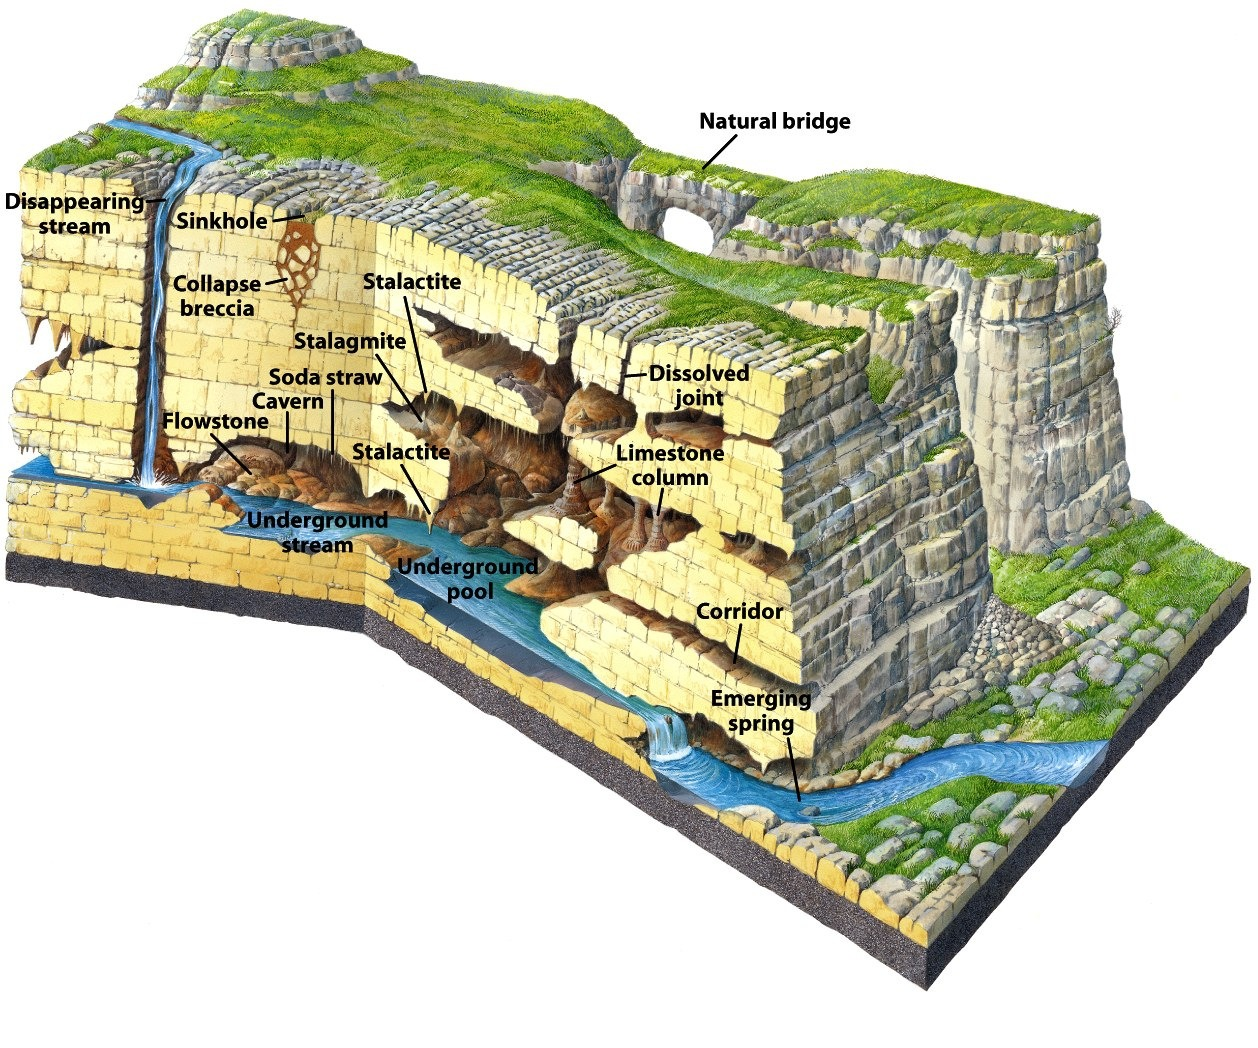
\includegraphics[width=1.2\textwidth]{chapters/karstification/karst_landscape.jpg}}
  \caption{Karst landscape showing various features of karst aquifers.
    Figure from \cite{marshak2006}}
  \label{fig:karstlandscape}
\end{figure}

\todo{Write about karst formations}

\section{Overview of karstification process}

\begin{figure}
  \centerline{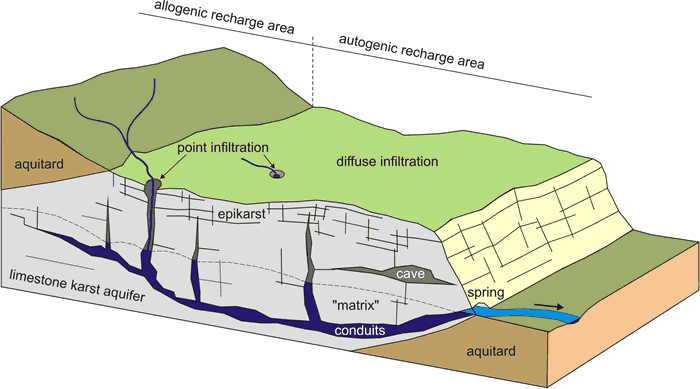
\includegraphics[width=\textwidth]{chapters/karstification/karstification.png}}
  \caption{Example of limestone karst aquifer.
    Figure from \cite{golscheider2007methods}}
  \label{fig:karstification}
\end{figure}

Most important factor in karstification process is flow of solvent throught an
underground aquifer. Since bedrock is subject to geological processes, a
net (sometimes called a matrix) of fractures of varying diameter and shape is
present in it. This solvemt, usually waterm flows through this kind of net
reacts with rock in ways described later.

Such karst aquifer may be surrounded on its sides by an aquitart, a substance
that is impenetrable to the water.

Water that enters the system may come from precipation, rivers or lakes. Inflow
of the water may happen through diffuse infiltration or point infiltration.
Diffuse infiltration happens on larger areas, covered by small fractures whereas
point infiltration requires a prominent fracture to be present in the aquifer
that can take large amounts of water from a river or lake.

Recharge water that comes to the karst aquifer from neighbouring non-karst areas
is called \emph{allogenic recharge}. For example on figure~\ref{fig:karstification}
a river flowing on the upper aquitard and entering the limestone aquifer through
the sinkhole is an allogenic recharge.

On the other hand, recharge water that flows directly to the karst area e.g. by
precipation is called an \emph{autogenic recharge}

Water that flows through the aquifer reacts chemically with walls of the
fractures widening them through dissolution. After going through the aquifer,
water reemerges at lower level through emerging springs or resurgences.

There are also cases of ground formation resulting from human activity.
Although not truly a karst process, a sinkhole that opened in 2010 in city of
Guatemala was a result of combination of loose ground made of volcanic ash and
inadequate draining system, that couldn't dissipate large amounts of water
brought by tropical storm Agatha \parencite{times2010}.

\section{Limestone dissolution}

Chemical reactions that take place during the karstification process will be
shown for limestone aquifers. Following description is taken form \cite{dreybrodt2002}
which is based on \cite{plummer1978}.

As the rain passes throught the atmosphere, it's picking up carbon dioxide that
gets dissolved in water. During this dissolution, small amounts of carbonic acid
are produced:

\ce{H2O + CO2 -> H2CO3} \todo{describe reactions}

\ce{H2O + CaCO3 <-> Ca^2 + CO3^{2-} + H2O}

\section{Formation of speleothems}
